\chapter{Sample Applications}

Over the course of our project, we developed two sample applications, XDCinema and XDYouTube. While developing those applications, we used XDTools to test and debug them. Using XDTools while developing two real cross-device applications helped us gain further ideas for improving XDTools and served as a first evaluation step for XDTools. In the following, we describe the two sample applications and the insights we gained while developing them.

\section{XDCinema}

As the name suggests, XDCinema is a cross-device cinema application. It allows users to check the cinema listings and view different information about movies and cinemas. It can be used with one to four different devices. On the ``main device'', the user can specify a city and date. They will then see a list of movies that are shown in this city on that date. The application is split into four different views that can be seen in Figure~\ref{fig:xdcinema} and that all show different information:
\begin{itemize}
	\item The search view (a): In the search view, the movies shown in the selected city on the selected date are shown. For each movie, the cinemas in the selected city that show the movie and the times at which the movie is shown are displayed.
	\item The location view (b): In the location view, the location of the selected cinema is shown on a map. The location view is shown when the user clicks on a cinema in the search view.
	\item The movie view (c): In the movie view, information about the selected movie is displayed. It shows an image of the movie, the summary, the genres, the duration and the average rating of the movie. Furthermore, it displays a link to the trailer of the movie and the ticket prices in the cinemas in the selected city. If a cinema is selected, the price that corresponds to that cinema is highlighted. The movie view is shown when the user clicks on a movie in the search view.
	\item The trailer view (d): In the trailer view, the trailer of the selected movie is displayed. The trailer view is shown when the user clicks on the link to the trailer in the movie view.
\end{itemize}

\begin{figure}[H]
  \centering
    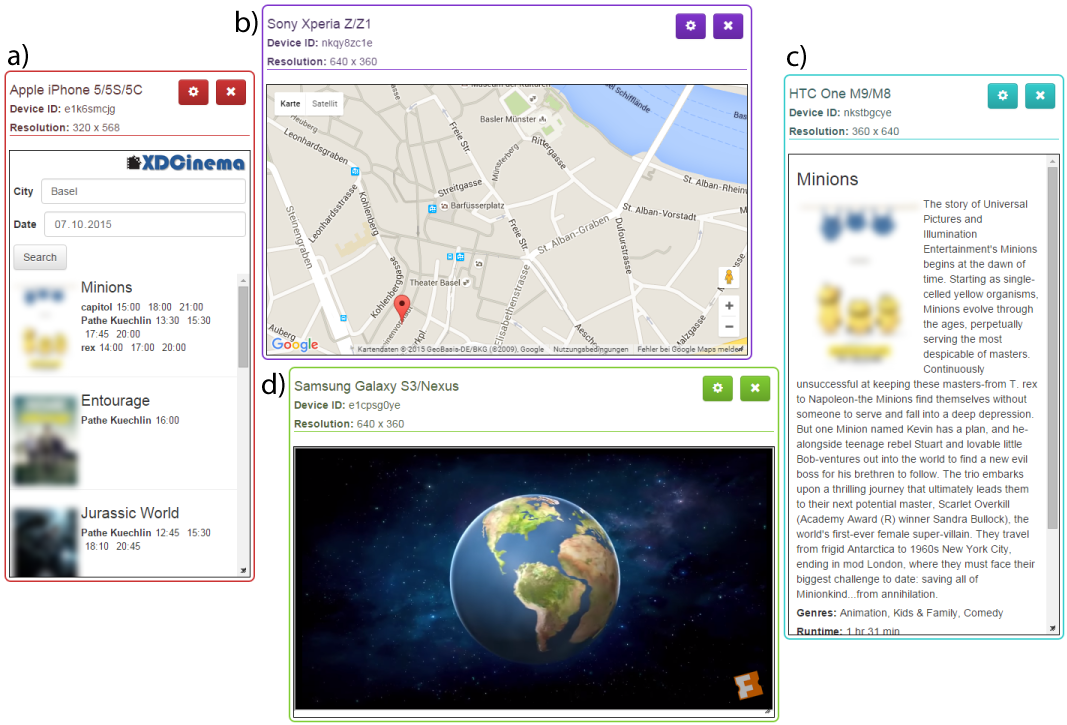
\includegraphics[width=1.0\textwidth]{images/screenshots/xdcinema_5_labeled.png}
	\caption[Screenshot XDCinema: Different views]{Different views of XDCinema}
	\label{fig:xdcinema}
\end{figure}

Depending on the number of devices that are connected, the four views are distributed differently. The trailer view is shown when the link to the trailer in the movie view is clicked and is only shown when at least four devices are connected. Otherwise, the link is just opened in a new tab on the device with the movie view. If only one device is connected, the remaining three views are all shown on that device and when the user navigates away from the search view they can get back to the search view using a back button. When two devices are connected, the movie view and the location view are both moved to the second device and the view that is shown depends on where the user last clicked in the search view. If the user clicks on a movie in the search view, the movie view is shown; if they click on a cinema, the location view is shown. If three devices are connected, the three views are distributed among all three devices. If more than four devices are connected, all additional devices also show the trailer view.

\subsection{Implementation}

XDCinema was implemented using the XD-MVC framework, but without Polymer. Thus, it is just a standard web application that accesses the JavaScript API of XD-MVC. Due to the difficulty of finding suitable APIs in the cinema and movie domain, the data that is used in the application is statically encoded in a JavaScript file. However, the application could easily be extended to support access to an API instead. The DOM on each device contains all four application views and all except the appropriate application view are hidden depending on the role of the device. 

Whenever a new device connects or a device disconnects, the roles are re-distributed and the views are updated. The available roles correspond to the four different views, thus the role assignment is performed according to the rules of the view distribution described above. The selected city, movie and cinema are synchronized between all connected devices through a shared variable using XD-MVC. When a shared variable is updated, each device performs the appropriate actions depending on its role. The selected city, movie, and cinema can only be changed from the search view. Therefore, all other devices only receive updates but do not send any updates themselves. If only one device is present, it has to hide the search view and location view if the selected movie is changed and it has to hide the search view and the movie view if the selected cinema changes. If the user wants to go back to the search view, it has to hide the location and movie view. If a device has both the movie and the location role, it has to hide the appropriate view when either the selected movie or the selected cinema changes. In cases where three or more devices are connected, the views that have to be hidden do not change and only the information in the view has to be updated if the respective shared variable changes. 

\section{XDYouTube}

XDYouTube is a cross-device YouTube application that allows multiple people to watch videos together on one large screen. The application allows users to search for videos on their devices and add them to a queue. The videos in the queue are played one after another on a large screen. The users can also look at the currently playing video and the queued videos or pause and play the current video from their devices. 

The application is split into two different views, the controller view and the player view. In the player view (see Figure~\ref{fig:xdyt_player}), the current video is played. 

\begin{figure}[H]
  \centering
    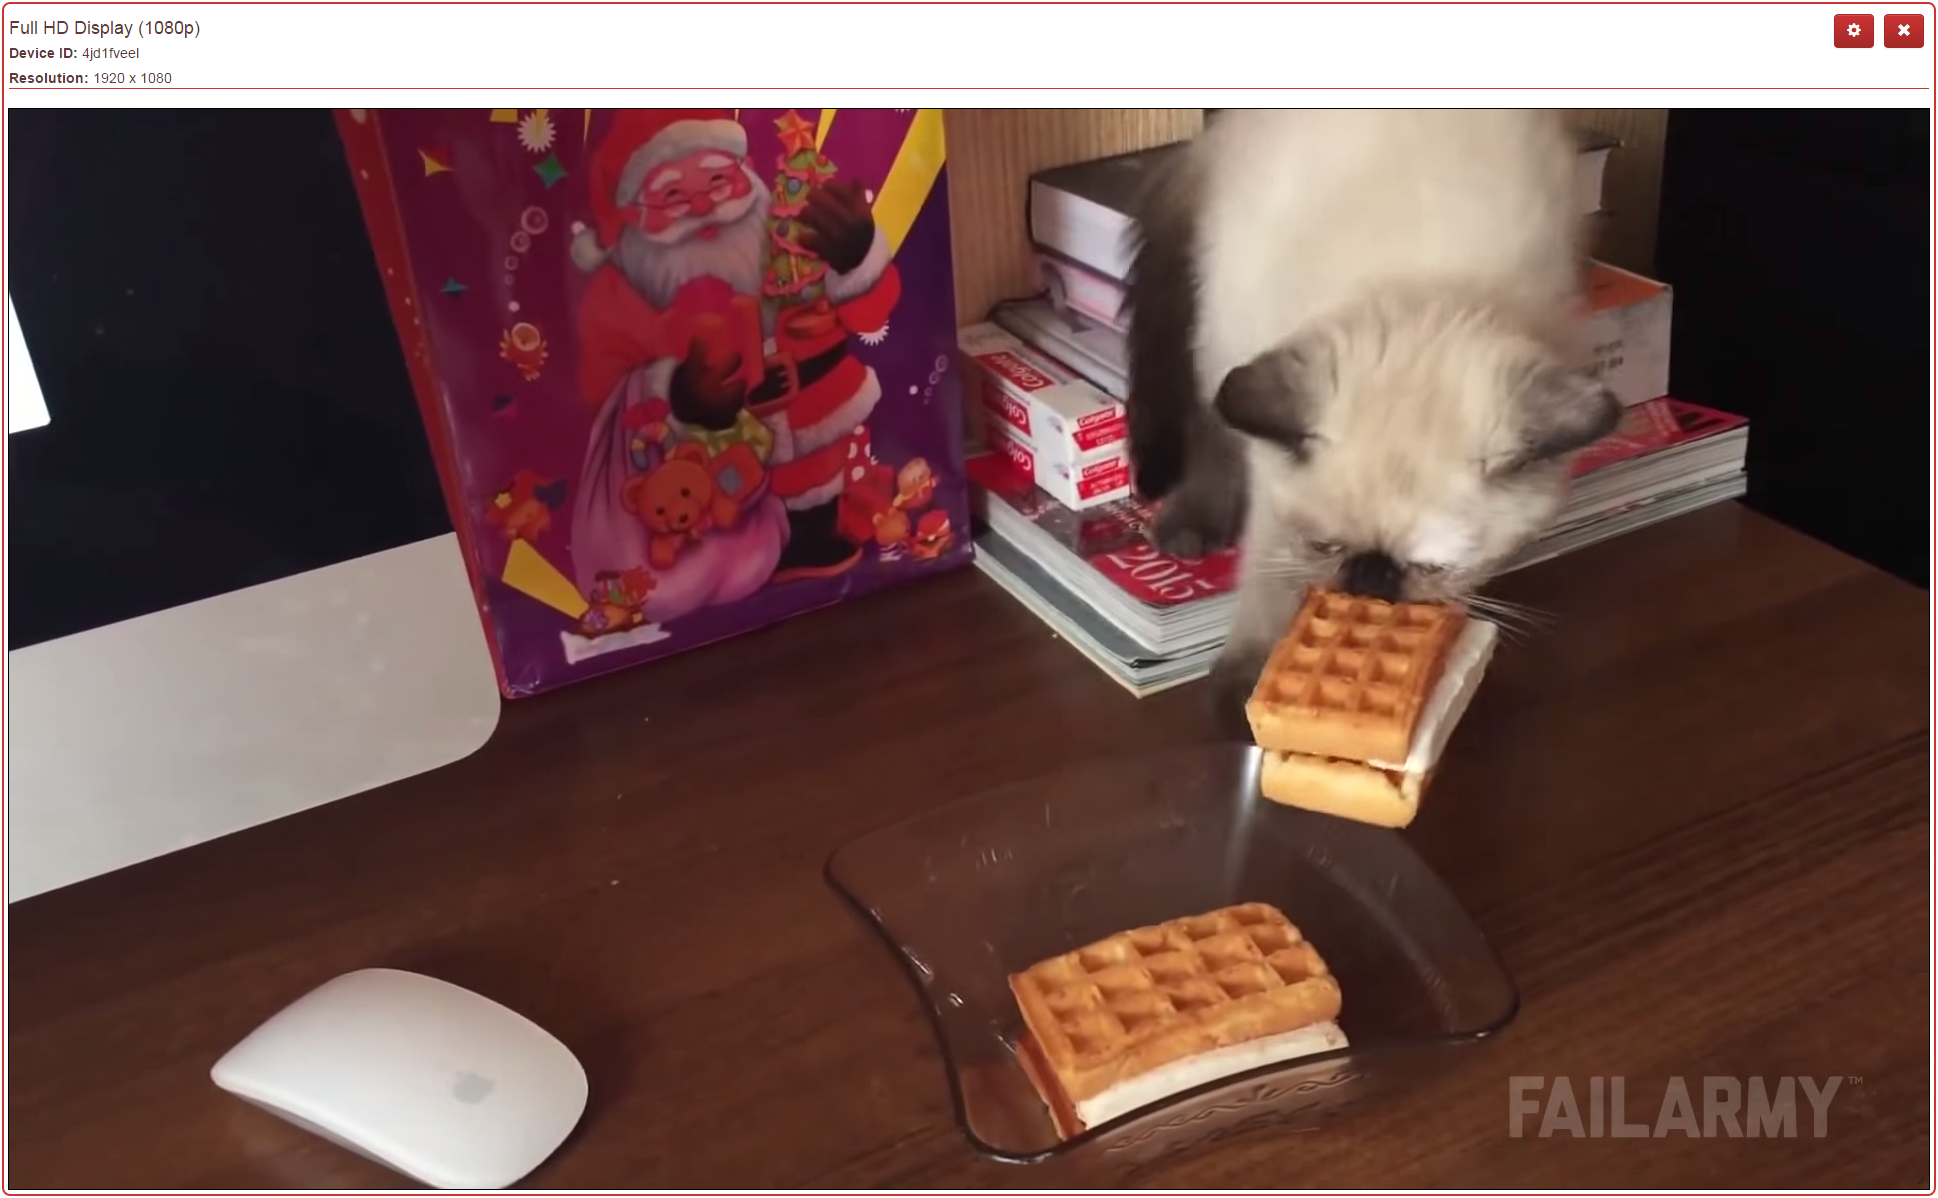
\includegraphics[width=0.8\textwidth]{images/screenshots/xdyt/player_2.png}
	\caption[Screenshot XDYouTube: Player view]{Player view of XDYouTube}
	\label{fig:xdyt_player}
\end{figure}

The controller view consists of two different parts:
\begin{itemize}
	\item In the first part, the user can search for videos. If the user searches for a video, a list of results is displayed. For each result, the thumbnail, title and description of the video is displayed. The user can click on a button to add the video to the queue. They can also navigate to the next page of search results.
	\item In the second part, the user sees the title, thumbnail and description of the current video. They can also pause or continue the video. The user also sees the thumbnails and titles of the videos that are still in the queue. 
\end{itemize}

On large devices, both parts of the controller view are displayed simultaneously. On smaller devices, the first part is only shown in portrait mode (see Figure~\ref{fig:xdyt_controller_portrait}). The second part is only shown in landscape mode (see Figure~\ref{fig:xdyt_controller_landscape}).

\begin{figure}[h!]
  \centering
    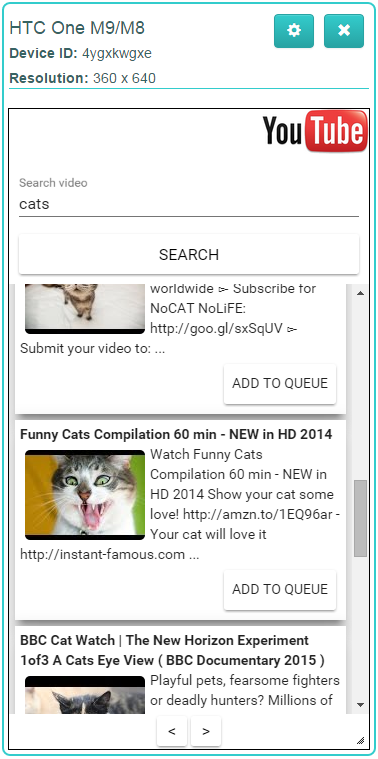
\includegraphics[width=0.3\textwidth]{images/screenshots/xdyt/controller_portrait_2.png}
	\caption[Screenshot XDYouTube: Controller view (first part)]{First part of the controller view in XDYouTube}
	\label{fig:xdyt_controller_portrait}
\end{figure}

\begin{figure}[h!]
  \centering
    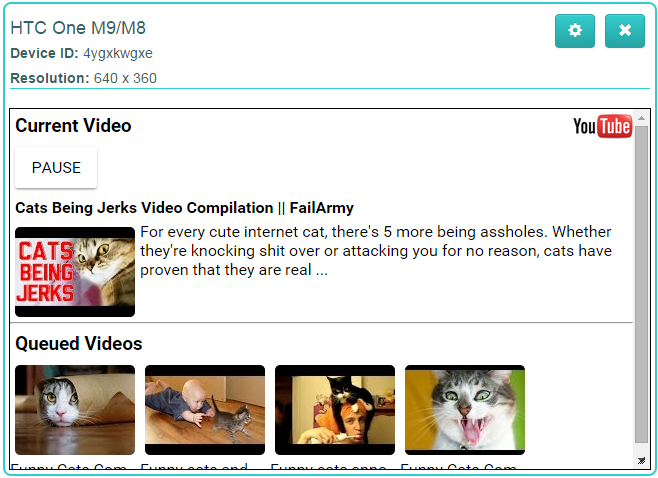
\includegraphics[width=0.7\textwidth]{images/screenshots/xdyt/controller_landscape_2.png}
	\caption[Screenshot XDYouTube: Controller view (second part)]{Second part of the controller view in XDYouTube}
	\label{fig:xdyt_controller_landscape}
\end{figure}

The device with the largest resolution automatically shows the player view. All other devices show the controller view. 

\subsection{Implementation}

XDYouTube is implemented with XD-MVC in combination with Polymer. The devices in the application can have three different roles:
\begin{itemize}
	\item ``player'': This role is assigned to the largest device.
	\item ``controller'': This role is assigned to all devices except the largest device.
	\item ``xlarge'': This role is assigned to devices with a width of more than 1000 pixels.
\end{itemize}
Depending on the role and the orientation of a device, different views are shown. As described above, the device with the role ``player'' shows the player view. Devices with the roles ``xlarge'' and ``controller'' show both parts of the controller view simultaneously, devices that only have the role ``controller'' show only one part of the controller view, depending on the orientation. When a new device connects or a device disconnects, the roles and the views are updated to reflect the new device configuration. The current video, the video queue and the video state (whether the video is playing or paused) are synchronized between devices. 

\section{Insights}

While developing the sample applications, we used XDTools. However, the implementation of XDTools was not complete yet at that point and some ideas only emerged while developing the applications. Before starting with the development of the applications, the devices had to be connected manually. During the development, we realized that constantly re-connecting devices is one of the most time-consuming tasks while developing cross-device applications. Thus, we came up with the idea of automatic connection management. Furthermore, we noticed that we often wanted to look at the JavaScript of the devices. But locating the correct file for a device was a difficult task, and the subdomains generated by our DNS server complicated things even more. We first had to look for the subdomain of the device, then locate the subdomain in the large list of domains in the browser debugging tools, and finally navigate to the file and code that we wanted to look at. This made it evident that some mechanism for opening files or functions on a specific device was required. Thus, we integrated function debugging into XDTools. 

Developing the sample applications also helped with locating and fixing some bugs. It also gave us some ideas for further improvements that are not yet included with XDTools. One example is the positioning of emulated devices: Right now, devices are always added in the top left corner of the device area. Therefore, the developer always has to move the device away from this location before creating the next device because otherwise the devices would overlap. Some algorithm that automatically looks for a free area where the emulated device can be placed would help solve this problem and make creating devices even more efficient.

In general, XDTools already helped a lot while developing the sample applications. Adding multiple emulated devices that do not share any local resources was probably the most useful feature of XDTools. However, the shared JavaScript console also proved helpful while developing the sample applications. We did not use record and replay very often during the development of the applications. In hindsight, we can think of a few situations where it might have been useful, but in that situation, we did not think about using record and replay. Record and replay is a feature that has not often been used previously by developers, and we did not use it before either, thus it might take some time to get used to it and recognize situations where it is useful. Furthermore, our sample applications are rather simple and did not require extensive debugging. However, as far as we can tell from our development experience, XDTools is very useful for testing and debugging a cross-device application.